%%%%%%%%%%%%%%%%%%%%%%%%%%%%%%%%%%%%%%%%%%%%%%%%%%%%%%%%%%%%%%%%%%%%%%%%%%%%%%%

\chapter{RELATED WORKS}\label{ch:corr}

In this section the related works will be presented, and they can be divided into two sections: the Big Data solutions from other operators, and the algorithms for the construction of data cubes with high cardinalities.

\section{Operations Data}\label{ch:corr:data}

\autoref{table:bigdatasattypes} shows the common data types used and generated by satellite operators, their origin and the common format for communication.
These data are either available to the satellite, or to the satellite operators in some way.

\begin{table}[!ht]
  \begin{center}
    \caption{Operations Data}\label{table:bigdatasattypes}
    \begin{tabular}{|c|C{5cm}|c|}
      \hline
      \bfseries Data Type & \bfseries Source           & \bfseries Format      \\
      \hline
      On-Board sensors & Satellite Equipment & Tables, CSV           \\
      \hline
      Computer Logs & On-Board computer& Text (\textit{Logs})  \\
      \hline
      Multimedia                     & Camera                    & MP4, JPG, RAW          \\
      \hline
      Orbital Parameters & Operations and Tracking & TLE, text, tables    \\
      \hline
      Associated documentation & Operators, Engineering  & Text (Word, Excel, PDF)    \\
      \hline
      Space Weather & Space or ground based information & Text, tables, warnings \\
      \hline
      Situational Awareness & Radars, US-STRACOM, etc   & CDM, text, tables, warnings \\
      \hline
    \end{tabular}
  \end{center}
  \FONTE{Adapted from~\cite{zhangBigDataFramework2017}}
\end{table}

For this work, only the data from the on-board sensors will be considered, as the other data in this table can considered for a larger data management effort by the operator organization, however they are out of scope.

\subsection{Data Flow}\label{ch:corr:dataflow}

Based on previous works and on the relevant data,~\autoref{fig:bigdataflow} shows a sample data flow expected of a Big Data architecture for satellite operators.
This flow is split into five phase that go from the source of the data to their final product analysis, and this work will only showcase the flow based on the correlated works, with each phase being:

\begin{figure}[ht]
  \caption{Data flow in a Big Data architecture}\label{fig:bigdataflow}
  \vspace{6mm}
  \begin{center}
    \resizebox{15cm}{!}{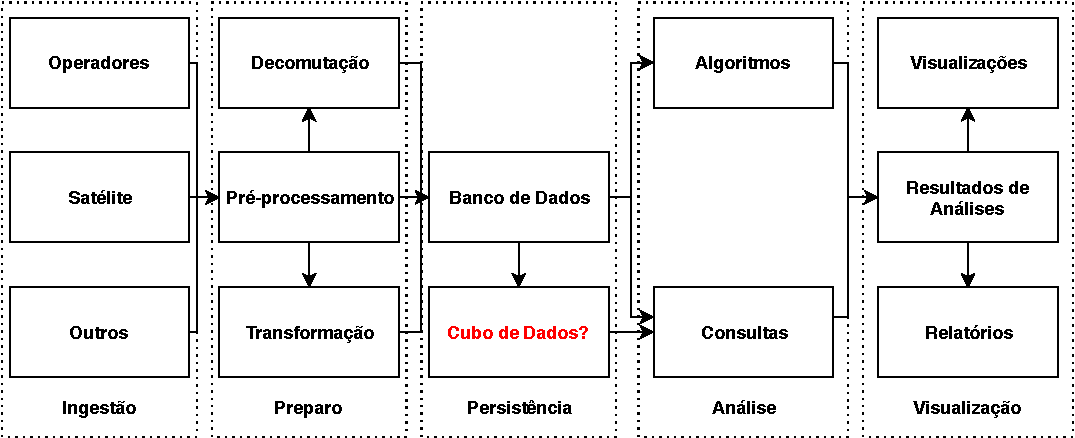
\includegraphics{Figuras/BigDataFlow.pdf}}
  \end{center}
  \vspace{2mm}
  \legenda{}
  \FONTE{Adapted from~\cite{zhangBigDataFramework2017}}.
\end{figure}

\RED{
  Can't find the original source. Working on it.
}

\begin{itemize}[noitemsep]
  \item \textbf{Collection}: where the data are collected at their source (satellite, ground sensors, etc).
    This phase treat \textbf{where} and \textbf{how} to collect the data, as well as \textbf{which} data are important enough to be collected.
    The source here can be a third party, another department or available through other means.
  \item \textbf{Preparation}: the relevant data are selected and the necessary transformations to insert them into the database are peformed.
    This phase treats the specific format of the data, doing cleaning, quality control and relevance for analysis, among others.
    The objective is to guarantee the quality, relevance and adequacy of the data to the database.
  \item \textbf{Storage}: after processing, the high quality data are stored in a database, where they will be available for analysis.
    At this point any data storage means are used, treating only how these data are stored and how they will be available for analysis.
  \item \textbf{Analysis}: queries and algorithms will be executed on the data, with the assurance and availability of high quality data.
    This can range from simple queries (``what's the value of telemetry X during pass Y?''), to the use of complex algorithms (``predict the values of telemetry X for the next three passes on station Z'').
  \item \textbf{Presentation}: analysis and algorithmic results are displayed to their end users.
    These can range from simple graphs to complex reports, as well as the result of algorithms. Anything that reaches the decision makers.
\end{itemize}

The works of~\cite{zhangBigDataFramework2017},~\cite{mateikUsingBigData2017} and~\cite{boussoufBigDataBased2018} have this process the best well defined out of all presented articles.

\section{Data Analysis by Satellite Operators}\label{ch:corr:ops}

\autoref{table:bigdataoperators} shows some recent published work made by satellite operators about the architectures that they use to process and analyze satellite data.

\begin{table}[htbp]
  \begin{center}
    \caption{Satellite Operators and Big Data Architectures}\label{table:bigdataoperators}
    \begin{tabular}{|C{13em}|C{6em}|c|C{10em}|}
      \hline
      \bfseries Reference                           & \bfseries Operator & \bfseries Tool & \bfseries Technologies                                                                \\
      \hline
      \cite{adamskiDataAnalyticsLarge2016}           & L3 (EUA)           & InControl            & Hadoop, Spark, HBase, MongoDB, Cassandra, Amazon AWS                                 \\
      \hline
      \cite{boussoufBigDataBased2018}                & Airbus             & Dynaworks            & Hadoop, Spark, HDFS, HBase, PARQUET, HIVE                                            \\
      \hline
      \cite{dischnerCYGNSSMOCMeeting2016}            & SwRI + NOAA        & CYGNSS MOC           & SFTP, -                                                                              \\
      \hline
      \cite{edwardsDealingBigData2018}               & EUMETSAT           & MASIF                & FTP, RESTful service, JMS Messague Queue, PostgreSQL                                 \\
      \hline
      \cite{evansDataMiningDrastically2016}          & S.A.T.E + ESA/ESOC & -                    & Java, CSV                                                                            \\
      \hline
      \cite{fenManagementOperationCommunication2016} & CSMT (China)       & -                    & - \\
      \hline
      \cite{fernandezTelemetryAnomalyDetection2017}  & NASA               & MARTE                & R, CSV, ad-hoc                                                                       \\
      \hline
      \cite{gillesFlyingLargeConstellations2016}     & L-3                & InControl            & Amazon EC2, LXC, Nagios                                                              \\
      \hline
      \cite{hennionBigdataSatelliteYearly2018}       & Thales Alenia      & AGYR                 & Logstash, Kafka, InfluxDB, ElasticSearch, Kibana, Grafana                            \\
      \hline
      \cite{mateikUsingBigData2017}                  & Stinger, NASA      & -                    & Logstash, ElasticSearch, Kibana, HDF5, CSV, R, Python, AWS, Excel                    \\
      \hline
      \cite{schulsterCHARTingFutureOffline2018}      & EUMETSAT           & CHART                & MATLAB, MySQL, Oracle                                                                \\
      \hline
      \cite{trollopeAnalysisAutomatedTechniques2018} & EUMETSAT           & CHART                & ad-hoc algorithms, a case study only \\
      \hline
      \cite{yvernesCopernicusGroundSegment2018}      & Telespazio France  & PDGS                 & OLAP (DataCube), Saiku, Pentaho, Jaspersoft OLAP                                     \\
      \hline
      \cite{zhangBigDataFramework2017}               & SISET (China)      & -                    & Hadoop, HDFS, PostgreSQL, MongoDB, Logstash, Kibana, ElasticSearch, Kafka, MapReduce \\
      \hline
    \end{tabular}
  \end{center}
  \FONTE{Author.}
\end{table}

The common objective in these is to ease the satellite operator activities by means of anomaly detection algorithms and telemetry bounds checking.
Some operators in this list are responsible for constellations of complex satellites, like remote sensing and communications, which are only cost-effective with a certain degree of automation for continuous operations.

These articles are filtered by only technologies that are used by the operators and not necessarily by the mission exploitation, as the housekeeping telemetry is on a different data ingestion pipeline than the payload data, as shown in~\cite{mateikUsingBigData2017} and~\cite{adamskiDataAnalyticsLarge2016}.

Some of these do not shown complete infrastructure for the entire data flow, like~\cite{fernandezTelemetryAnomalyDetection2017} and~\cite{trollopeAnalysisAutomatedTechniques2018} that use \textit{ad-hoc} scripting, and focus on only one part of the data flow.

In~\cite{yvernesCopernicusGroundSegment2018} the authors showcase some OLAP queries and the use of a data cube, having used dimensional modelling to aid the operation of a satellite constellation. However, this work only showcases at a very high level the used methodology, and mention that the work was performed only on at the modelling level to be integrated with other tools, not showcasing the rest of the infrastructure needed for this to work.

\subsection{Data Analysis at INPE}\label{ch:corr:inpe}

INPE already perform data analysis on satellite telemetry, and in fact in many departments other than satellite operations.
The satellite operators must monitor the telemetries, analyse the incoming data, and act based on engineering guidance in case a problem is identified~\cite{TominagaFerrAmbr:2017:CoSaTe}.
An example is in~\cite{Magalhaes:2012:EsAvTe}, made about a fault on the CBERS-2 satellite, where the proposed model would enhance knowledge about a phenomenon known as thermal avalanche that can make a satellite inoperable and thus identify and be able to stop that from happening again.
Furthermore, as in line with~\autoref{table:bigdataoperators}, anomaly detection is a common area of study~\cite{AzevedoAmbrViei::EsSoTe}.

Other departments will mostly use data from the payload or from external agents, like remote sensing data, which analysis is also not trivial and are definitely a Big Data problem.
\citeonline{monteiroFRAMEWORKTRAJECTORYDATA2017} use Big Data concepts to the trajectory analysis;~\citeonline{ramosDistributedSystemsPerformance2016} showcase the use of tools like Hadoop to analyse Space Weather data, and~\citeonline{SimoesCamaQuei:2018:DaAnMa} show an architecture based on data cubes for remote sensing time series analysis, to name a few.

\section{Data Cube Computation}\label{ch:corr:cube}

The selective computation of data cubes has a rich history, due to the curse of dimensionality, most algorithms need a way to treat high dimensional data and deal with limited available memory~\cite{hanDataMiningConcepts2011}.

The \textit{Frag-Cubing} algorithm~\cite{liHighdimensionalOLAPMinimal2004} uses \textit{cube shells}, where subcubes with few dimensions (generally from 2 to 5) will be computed using an inverted index, thus using the fragments as a compromise between used memory and how many dimensions can be answered with a multidimensional query.
Frag-Cubing is one of the most efficient and popular data cube computation algorithms, and it's internal workings will be explored in the next section.

Using distributed computing,~\cite{dokaBrownDwarfFullydistributed2011} shows the Brown Dwarf, a Peer-to-Peer system that allows for cells to be updated and to reduce the redundancy in distributed cubes.

PopUp-Cubing is shown in~\cite{heinePopUpCubingAlgorithmEfficiently2017}, using icebergs to deal with streaming data, and having superior results to FTL and Star-Cubing.
This work specially deals with streaming data, which is of interest for real time data analysis of telemetries, however that that is not an scenario explored by this work.

Using MapReduce as a base, ~\cite{wangScalableDataCube2013} presents HaCube, seeking a balance between parallel cube computation between various MapReduce nodes, allowing updates and incremental computation of measures.
Due to its own distributed nature, it needs some fault tolerance to work, and also the tests were limited to only 5 dimensions, with up to 2,4 billion tuples.
Also using MapReduce \citeonline{yangHolisticAlgebraicData2017} demonstrates the computing of holistic measures by presenting Multi-RegionCube, however with less testing than the previous method.

In~\cite{zhaoClosedFragShellsCubing2018} it is presented Closed Frag-Shells Cubing, which combines the C-Cubing approach~\cite{dongxinCCubingEfficientComputation2006} of creating closed cube cells that losslessly compress drill-down/roll-up semantics, with the Frag-Cubing approach of using shell fragments, adding their own bitmap-based indexing on top to enhance query response times.
This work is probably the closest to this own thesis, however with much less implementation requirements.

\textit{qCube}~\cite{silvaQCubeEfficientIntegration2013} extend the Frag-Cubing approach by adding value interval queries, allowing for other comparison operators besides equality to be used in queries.
\textit{HFrag}~\cite{silvaHybridMemoryData2015} uses of external memory to aid in the computation of the inverted index, using a hybrid system to partition the cube in both main and secondary memory by keeping the most frequent used values in the main memory and the least used in the secondary memory.
Hybrid Inverted Cubing (HIC)~\cite{silvaComputingBIGData2016} is an extension to the HFrag algorithm that uses a critical accumulated frequency parameter, which ends up having better results in practice.

Of these works \textit{Frag-Cubing} keeps being a base robust algorithm to compute the cube, as the inverted index techniques are still relevant and the results are adequate.
However, \citeonline{liHighdimensionalOLAPMinimal2004} show the exponential memory usage of the different cube computation schemes using only 12 dimensions, and there is a clear saturation when cubes with 20, 50, 100 or more dimensions are used to compute the cube~\cite{silva:2015:abordagensParaCubo}.

\subsection{\textit{Frag-Cubing}}\label{ch:corr:cube:frag}

Therefore, this work will focus on ways of improving the performance of the Frag-Cubing algorithm, both in query response time and memory usage.
For that, it is necessary to understand how the algorithm computes the cube and answer queries.
It does this by using the concept of an inverted index, where each inverted tuple $iT$ has an attribute value, an Tuple Identifier (TID) list, and some computed measure values.
For example, let us consider four tuples: $t_1 = (tid_1, a_1, b_2, c_2, m_1)$, $t_2 = (tid_2, a_1, b_3, c_3, m_2)$, $t_3 = (tid_3, a_1, b_4, c_4, m_3)$, and $t4 = (tid_4, a_1, b_4, c_1, m_4)$.
These four tuples will generate eight inverted tuples: $iTa_1, iTb_2, iTb_3, iTb_4, iTc_1, iTc_2, iTc_3$ and $iTc_4$, shown in \autoref{fig:fragexample}.

For each attribute value an occurrence list is built, so for $a_1$ there is $iTa_1 = (a_1, tid_1, tid_2, tid_3, tid_4, m_1, m_2, m_3, m_4)$ where the attribute value 1 is associated with TIDs: $tid_1, tid_2, tid_3,$ and $tid_4$.
Tuple identifier $tid_1$ has the measure value $m_1$, $tid_2$ has the measure value $m_2$ and so on.
Query $q = (a_1, b_4, COUNT)$ can be answered by intersecting the lists $iTa_1 \cap iTb_4 = (a_1b_4, tid_3, tid_4, COUNT(m_3, m_4))$, in which $q, iTa_1 \cap iTb_4$ indicates the common TIDs between $iTa_1$ and $iTb_4$, their set intersection.

\begin{figure}[!htb]
  \caption{Inverted Index computation example}\label{fig:fragexample}
  \vspace{2mm}
  \begin{center}
    \resizebox{15cm}{!}{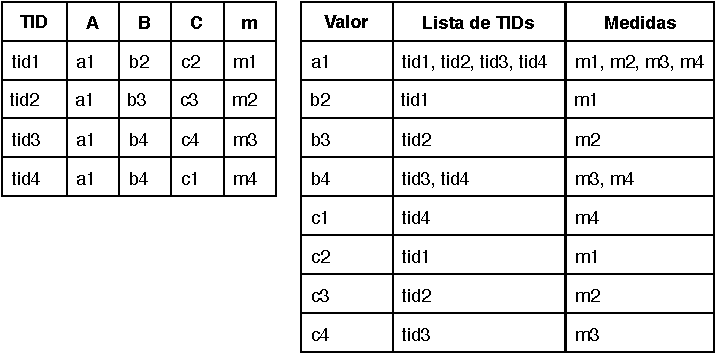
\includegraphics{Figuras/FragDrawing.pdf}}
  \end{center}
  \vspace{1mm}
  \legenda{}
  \FONTE{Author.}
\end{figure}

\RED{Can't find this source, I'll update it later}

The complexity of the intersection is proportional to the number of times that an attribute value occurs in the input data, but bounded by the size of the smallest list, and in this example $iTb_2$ with a single TID is the smallest list.
The number of TIDs associated to an attribute value can then be enormous, with low cardinality dimensions and high number of tuples needing a high processing capacity.
Smaller TID lists allow for queries to be quickly answered, so relations with a low skew, or uniformity of values in the relation attributes, and high cardinality are more suitable to be computed by approaches with Frag-Cubing.

Furthermore, a skew close to zero can indicate a relation with uniformly distributed values, and the higher this value the less uniform the relation list will be.

The algorithm also introduces the concept of cube shells: instead of computing every combination of low-dimensional cubes, only a thin shell of dimensions is computed.
This translates to dividing the number of dimensions in the data by the supplied fragment size parameter $\mathcal{F}$ and generating all subcubes with that amount of dimensions, but not repeating the dimensions that have already been generated.
\autoref{fig:hasseexample} shows a typical full cube with three dimensions $A, B$ and $C$, with the top being the raw cell data ($0$-dimensional cube) and the base being the most aggregated cell that summarizes all data.

If we set $\mathcal{F} = 1$, then the Frag-Cubing algorithm will only pre-compute dimensions $A, B$ and $C$, as they are the lowest dimensions that fit the fragment size, as is the standard of a cube that doesn't compute any aggregation besides the single dimensions.
However, if we set $\mathcal{F} = 2$, then the algorithm will compute from left to right the subcube $\{A, B\}$, then see that there aren't enough dimensions for another cube with the same size as the fragment and compute the next remaining not computed subcube $\{C\}$, thus computing the subcubes $[\{A, B\}, \{C\}]$.
If $\mathcal{F} = 3$, then the full cube would be precomputed, equating a fully materialized cube with all children subcubes being computed too.

\begin{figure}[!htb]
  \caption{Shell Fragmentation example}\label{fig:hasseexample}
  \vspace{2mm}
  \begin{center}
    \resizebox{8cm}{!}{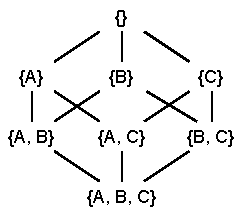
\includegraphics{Figuras/FragCubing-HasseBase.pdf}}
  \end{center}
  \vspace{1mm}
  \legenda{}
  \FONTE{Author.}
\end{figure}

